\documentclass[11pt]{article}

% parameters are fairly self-explanatory here, thankfully
\usepackage[width=7in,height=9.5in,top=0.75in,centering]{geometry}

% for math-ing
\usepackage{amsmath}
\usepackage{amssymb}


%%%%%% tables %%%%%%%%

\usepackage{array}
\renewcommand{\arraystretch}{1.5}
\setlength{\tabcolsep}{8pt}

%%%%%% plotting %%%%%%

\usepackage[dvipsnames]{xcolor}
\usepackage{tikz}
\usepackage{pgfplots}

\pgfplotsset{every axis/.append style={
                    axis x line=middle,    % put the x axis in the middle
                    axis y line=middle,    % put the y axis in the middle
                    axis line style={<->,color=black}, % arrows on the axis
                    xlabel={$x$},          % default put x on x-axis
                    ylabel={$y$},          % default put y on y-axis
            }}
            
 \pgfplotsset{compat=1.14} % sometimes, everything falls apart without this
 
 %\usepgfplotslibrary{fillbetween} %for shading between curves

%%%%%% commands %%%%%%

% exam heading; course name is first argument, exam information is second argument
\newcommand{\Heading}[2]{
    \fbox{
        {\Large\textbf{#1}}
        }
    \hfill
    \fbox{
        \begin{minipage}{0.2\textwidth}
            \begin{center}
            \textbf{#2}
            \end{center}
        \end{minipage}
    }
    \par\vspace{0.1in}}

% for being lazy while beautifying integrals
\newcommand{\dint}{\displaystyle\int}

% for being lazy while beautifying limits
\newcommand{\dlim}{\displaystyle\lim}

%%%%%% stuff %%%%%%

\usepackage{fancyhdr}

%\setcounter{page}{0} % first page is page 0

\parindent0pt % no indent

\fboxsep=0.25cm % little space in fbox border

%%%%%% BEGIN! %%%%%%%

\begin{document}

\pagestyle{fancy}

% record goals here to create sense of transparency

\fancyhead[c]{%
  \ifcase\value{page}
  % empty test for page = 0
  \or {}% 
  \or
  \or {\bf\color{ProcessBlue} F1: Lines \& Slope}% page=1
  \or {\bf\color{ProcessBlue} F2: Exponential and Logarithmic Functions}% page = 2
  \or {\bf\color{RoyalBlue} L2: Evaluating Limits Using Continuity and Forms}% page = 3
  \or {\bf\color{RedOrange} A1: Derivatives and Graphing}% page = 4
  \or {\bf\color{RedOrange} A2: Local and Absolute Extreme Values}% page = 5
  \or {\bf\color{RedOrange} A3: Applied Optimization}% page = 6
  \or {\bf\color{Fuchsia} I2: Properties of Definite Integrals}% page = 7
    \or {\bf\color{Fuchsia} I2: Properties of Definite Integrals}% page = 8
  \or {\bf\color{Fuchsia} I3: Antiderivatives and Indefinite Integrals}% page = 8
  \or {\bf\color{Fuchsia} I4: Compute Definite Integrals}
  \else
  % Empty chead here!
  \fi
}

\thispagestyle{empty} % don't display that this is page 0

\Heading{MATH 1190/1210 Survey of Calculus I}{Final Exam\\Growth-Based\\Fall 2025\\Part 2}

\vspace{0.1in}

\textbf{Name} \hrulefill \, \begin{minipage}{0.16\textwidth}\begin{center}\textbf{UVA ID\\ (e.g. hdj4nd)} \end{center}\end{minipage}\hrulefill\\

\begin{minipage}{0.2\textwidth}\begin{center}\textbf{Course \&\\ Section Number} \end{center}\end{minipage} \hrulefill\,\,\textbf{Date} \hrulefill  \\

\hrulefill
\paragraph*{Course \& Section Numbers:}

{\small
\begin{center}
\begin{tabular}{| c | c | c | c | c |}
\hline
%
\begin{minipage}{0.12\textwidth}\begin{center}
1190-100\\
J. Rolf\\
(11:00 AM)
\end{center}\end{minipage}
&
\begin{minipage}{0.12\textwidth}\begin{center}
1190-200\\
J. Rolf\\
(9:30 AM)
\end{center}\end{minipage}
&
\begin{minipage}{0.12\textwidth}\begin{center}
1210-100\\
Mikhail\\
(8 AM)
\end{center}\end{minipage}
&
\begin{minipage}{0.12\textwidth}\begin{center}
1210-200\\
Raul\\
(9:30 AM)
\end{center}\end{minipage}
&
\begin{minipage}{0.12\textwidth}\begin{center}
1210-300\\
Sherman\\
(11 AM)
\end{center}\end{minipage}
\\
%
\hline
%
\begin{minipage}{0.12\textwidth}\begin{center}
1210-400\\
Sherman\\
(12:30 PM)
\end{center}\end{minipage}
&
\begin{minipage}{0.12\textwidth}\begin{center}
1210-500\\
Michael\\
(2 PM)
\end{center}\end{minipage}
&
\begin{minipage}{0.12\textwidth}\begin{center}
1210-600\\
J. Bowling\\
(3:30 PM)
\end{center}\end{minipage}
&
\begin{minipage}{0.12\textwidth}\begin{center}
1210-700\\
Josh\\
(9:30 AM)
\end{center}\end{minipage}
&
\begin{minipage}{0.12\textwidth}\begin{center}
1210-800\\
Mason\\
(2 PM)
\end{center}\end{minipage}
\\
%
\hline
%
\begin{minipage}{0.12\textwidth}\begin{center}
1210-900\\
Caelan\\
(3:30 PM)
\end{center}\end{minipage}
&
\begin{minipage}{0.12\textwidth}\begin{center}
1210-920\\
Caelan\\
(5 PM)
\end{center}\end{minipage}
&
\begin{minipage}{0.12\textwidth}\begin{center}
1210-940\\
Mitchell\\
(10 AM)
\end{center}\end{minipage}
&
\begin{minipage}{0.12\textwidth}\begin{center}
1210-950\\
Mitchell\\
(11 AM)
\end{center}\end{minipage}
&
\begin{minipage}{0.12\textwidth}\begin{center}
1210-960\\
Mitchell\\
(noon)
\end{center}\end{minipage}
\\
\hline
\end{tabular}
\end{center}

}

{%\small

\paragraph*{Instructions:}

\begin{itemize}
    
    \item The regular time allowed for completing this assessment is \fbox{$80$} minutes.
    \item \textbf{This part of the final exam is optional.} It provides one additional opportunity to attempt the following learning targets.
    {\bf\color{ProcessBlue}F1}, {\bf\color{ProcessBlue}F2}, {\bf\color{RoyalBlue}L2}, {\bf\color{RedOrange}A1}, {\bf\color{RedOrange}A2}, {\bf\color{RedOrange}A3}, {\bf\color{Fuchsia}I2}, {\bf\color{Fuchsia}I3}, {\bf\color{Fuchsia}I4}.
    %\item This assessment is out of 50 points.\\
    \item On each problem, you will receive a score of Exceeds Expectations (5), Proficient (4), Almost (3), Developing (2), Emerging (1), or Not Yet (0). {\bf Please do not interpret your score as a percentage.}
    %\item You will have opportunities to reassess on the targets appearing on this assessment after the next {\bf 2} assessments.\\
    \item You may NOT use calculators, dictionaries, notes, phones, or any other kind of aid.
    \item Please write neatly. What cannot be read, cannot be graded.
    \item Carefully work out each problem and clearly indicate your final answer to every problem.
    \item Throughout, give the most descriptive answer possible. \textbf{For instance, ``DNE" will not be accepted when ``$=\infty$" is applicable.}
    %\item Please provide the most specific answer possible. For instance, if a limit does not exist because it goes to $\infty$ or $-\infty$, then specify this.
    \item Please use the methods discussed up to this point in the course. For example, any work based on l'H\^opital's Rule will not receive credit.
    \item \textbf{All work must be shown unless otherwise specified.} Partial credit will not be given if appropriate work is not shown.
    \item In particular, {\bf any answer appearing with no justification will receive no credit regardless of whether the answer was correct}, unless otherwise specified.
    \item Please first respond to the prompts on which you feel most proficient, then respond to others later.
    \item This booklet is printed double-sided. It contains 14 pages and 9 numbered problems.
    \end{itemize}
    
    }

\vfill


%%%%%%%%%
\newpage

This page is left blank intentionally.\\

Use this page if you need additional space to write your solutions to any problem. \\

If you wish this page graded, you must refer to this page on \textbf{the original page} of the problem. Otherwise, your grader will NOT consider your work on this page.

\newpage%
%%%%%%%%%


\begin{enumerate}

%%%%%%%%%%%%%%%%%%%%%%%%%%%%%%%%%%%%%%%%%%%%%%%%%%%%%
%%%%%%%%%%% BEGIN PROBLEM F1 %%%%%%%%%%%%%%%%%%%%%%%%
%%%%%%%%%%%%%%%%%%%%%%%%%%%%%%%%%%%%%%%%%%%%%%%%%%%%%

\item The wind chill factor (in $^\circ F$) is a function of the wind speed (in miles/hour). Below is a table relating these two quantities.

    \begin{table}[h!]
        \centering
        \begin{tabular}{c|ccccc}
            \hline
           Wind Speed  & 5 & 10 & 15 & 20 & 25 \\
           \hline
           Wind Chill Factor & 16 & 3 & -5 & -10 & -15\\
           \hline
        \end{tabular}
    \end{table}

\begin{enumerate}
    \item When the wind speed changes from $5$ miles/hour to $15$ miles/hour, what is the net change in the wind chill factor?

    \vfill

    \item  Find the average rate of change of the wind chill factor when the wind speed changes from $10$ miles/hour to $25$ miles/hour.
    
    To receive full credit, please make sure to include appropriate units.

    \vfill
    \vfill

    \item Use a sentence or two to explain the meaning of the average rate of change found in part (b) \textbf{in the context of this scenario}. 

    Note: Simply stating the ``slope" is the ``average rate of change" of the relevant quantities will not receive credit. You must explain the meaning of the average rate of change using the details and quantities related to the context of this question.

    \vfill
    \vfill
\end{enumerate}

%%%%%%%%%%%%%%%%%%%%%%%%%%%%%%%%%%%%%%%%%%%%%%%%%%%%%
%%%%%%%%%%% END PROBLEM F1 %%%%%%%%%%%%%%%%%%%%%%%%%%
%%%%%%%%%%%%%%%%%%%%%%%%%%%%%%%%%%%%%%%%%%%%%%%%%%%%%

\newpage

%%%%%%%%%%%%%%%%%%%%%%%%%%%%%%%%%%%%%%%%%%%%%%%%%%%%%
%%%%%%%%%%% BEGIN PROBLEM F2 %%%%%%%%%%%%%%%%%%%%%%%%
%%%%%%%%%%%%%%%%%%%%%%%%%%%%%%%%%%%%%%%%%%%%%%%%%%%%%
\item Respond to the following prompts.

\begin{enumerate}

\item Evaluate the following expressions. Simplify as much as possible. Your final answer should be a number without any exponential or logarithmic expressions.

\begin{enumerate}

\item[(i)] $\displaystyle \frac{(-2)^{-70}}{(-2)^{-66}}$

\vfill

\textcolor{blue}{
\[
\frac{(-2)^{-70}}{(-2)^{-66}}
= (-2)^{-70 - (-66)}
= (-2)^{-4}.
\]
Since $(-2)^4 = 16$, it follows that
\[
(-2)^{-4} = \frac{1}{16}.
\]
}

\vfill

\item[(ii)] $\displaystyle \log_{4}\!\left(\sqrt[5]{16^2}\right)$

\vfill

\textcolor{blue}{
First rewrite the expression using exponents:
\[
\sqrt[5]{16^2} = (16^2)^{1/5} = 16^{2/5}.
\]
Since $16 = 4^2$, we have
\[
16^{2/5} = (4^2)^{2/5} = 4^{4/5}.
\]
Therefore,
\[
\log_{4}(4^{4/5}) = \frac{4}{5}.
\]
}

\vfill

\end{enumerate}

\item Solve the following equation for $x$.

\[
11^{3x+2} = 5
\]

\vfill

\textcolor{blue}{
Take $\log_{11}(x)$ of both sides:
\[
\log_{11}\left(11^{3x+2}\right) = \log_{11}(5).
\]
Using the cancellation rule for logarithms,
\begin{align*}
3x+2 &= \log_{11}(5)\\
\end{align*}
Solve for $x$:
\[
3x+2 = \log_{11}(5)
\quad
3x = \log_{11}(5) - 2,
\quad
x = \frac{1}{3}\left(\log_{11}(5) - 2\right).
\]
}

\vfill

\end{enumerate}

%%%%%%%%%%%%%%%%%%%%%%%%%%%%%%%%%%%%%%%%%%%%%%%%%%%%%
%%%%%%%%%%% END PROBLEM F2 %%%%%%%%%%%%%%%%%%%%%%%%%%
%%%%%%%%%%%%%%%%%%%%%%%%%%%%%%%%%%%%%%%%%%%%%%%%%%%%%

\newpage

%%%%%%%%%%%%%%%%%%%%%%%%%%%%%%%%%%%%%%%%%%%%%%%%%%%%%
%%%%%%%%%%% BEGIN PROBLEM L2 %%%%%%%%%%%%%%%%%%%%%%%%
%%%%%%%%%%%%%%%%%%%%%%%%%%%%%%%%%%%%%%%%%%%%%%%%%%%%%

\item Evaluate the following limits using a theorem about continuity or form.

If you use a theorem about continuity to evaluate a limit, to receive full credit, please provide sufficient explanation for why the theorem can be used. 

If you use form to evaluate a limit, to receive full credit, please list the form and show all steps. 

There's no need to simplify your final answer.

\begin{enumerate}
    \item $\lim\limits_{x\to\infty}\dfrac{x^2}{\ln(x)+e^x}$ %change to infty/infty,Exponential/polynomial/log?

    \vfill

    \item $\lim\limits_{x\to 2^+}\dfrac{1}{2-x}$

    \vfill
\end{enumerate}

%%%%%%%%%%%%%%%%%%%%%%%%%%%%%%%%%%%%%%%%%%%%%%%%%%%%%
%%%%%%%%%%% END PROBLEM L2 %%%%%%%%%%%%%%%%%%%%%%%%%%
%%%%%%%%%%%%%%%%%%%%%%%%%%%%%%%%%%%%%%%%%%%%%%%%%%%%%

\newpage

%%%%%%%%%%%%%%%%%%%%%%%%%%%%%%%%%%%%%%%%%%%%%%%%%%%%%
%%%%%%%%%%% BEGIN PROBLEM A1 %%%%%%%%%%%%%%%%%%%%%%%%
%%%%%%%%%%%%%%%%%%%%%%%%%%%%%%%%%%%%%%%%%%%%%%%%%%%%%

\item 

\begin{enumerate}
    \item Consider the following graph.

    \begin{center}
        
\includegraphics[scale=0.5]{Fall 2025/Final Exam/FinalA1.png}
    \end{center}

    \begin{enumerate}
        \item Suppose the given graph is the graph of $f'$. Write down the $x$-values of all inflection points of $f(x)$.

        {\large
        \[\text{Inflection points ($x$-value(s) only): } {\color{blue} x=1, 4}\]
        }

        \vfill
        
        \item Suppose the given graph is the graph of $f''$. Write down the $x$-values of all inflection points of $f(x)$.

        {\large
        \[\text{Inflection points ($x$-value(s) only): } {\color{blue} x=0, 2, 6}\]
        }

        \vfill
    \end{enumerate}

    \item A function $f$ satisfies that $f(3)=5$, $f'(3)=2$, and $f''>0$ for $x>3$. Which one(s) of the following are possible values of $f(5)$? 
    
    Select all that apply. No justification required. Correct answer gets full credit. 

    \begin{itemize}
        \item 10
        \item 7
        \item 12
        \item 9
    \end{itemize}

    {\color{blue} 10 and 12}

    \vfill
    \vfill
\end{enumerate}

%%%%%%%%%%%%%%%%%%%%%%%%%%%%%%%%%%%%%%%%%%%%%%%%%%%%%
%%%%%%%%%%% END PROBLEM A1 %%%%%%%%%%%%%%%%%%%%%%%%%%
%%%%%%%%%%%%%%%%%%%%%%%%%%%%%%%%%%%%%%%%%%%%%%%%%%%%%

\newpage

%%%%%%%%%%%%%%%%%%%%%%%%%%%%%%%%%%%%%%%%%%%%%%%%%%%%%
%%%%%%%%%%% BEGIN PROBLEM A2 %%%%%%%%%%%%%%%%%%%%%%%%
%%%%%%%%%%%%%%%%%%%%%%%%%%%%%%%%%%%%%%%%%%%%%%%%%%%%%

\item Consider the following function $f(x)$.% and its derivative.

\[f(x)=2x^{1/3}-x^{2/3}\]%x^3-3x^2+1\]%-(x-1)^4(15x^2+18x+7)\]

%\[f'(x)=10(1-x)^3(3x+1)^2\]

You are required to use methods we've learned in our course, such as the first derivative test, the second derivative test, the closed interval method, or the first derivative test for absolute extrema, to solve this problem. In addition, you need to make sure the method you use is suitable for the question.

\begin{enumerate}
    \item Find all critical numbers of $f(x)$.

    \vfill

    %\item For each critical number found in part (a), classify it as a local minimum, a local maximum, or neither. Fully justify your work.

    %\vfill

    \item Find the $x$-values of all absolute extrema of $f(x)$ on the interval $[-1, 8]$.


    \vfill
\end{enumerate}

%%%%%%%%%%%%%%%%%%%%%%%%%%%%%%%%%%%%%%%%%%%%%%%%%%%%%
%%%%%%%%%%% END PROBLEM A2 %%%%%%%%%%%%%%%%%%%%%%%%%%
%%%%%%%%%%%%%%%%%%%%%%%%%%%%%%%%%%%%%%%%%%%%%%%%%%%%%

\newpage

%%%%%%%%%%%%%%%%%%%%%%%%%%%%%%%%%%%%%%%%%%%%%%%%%%%%%
%%%%%%%%%%% BEGIN PROBLEM A3 %%%%%%%%%%%%%%%%%%%%%%%%
%%%%%%%%%%%%%%%%%%%%%%%%%%%%%%%%%%%%%%%%%%%%%%%%%%%%%

\item Find two real numbers differing by 20 whose product is as small as possible.

To receive full credit, please provide full justification of why the two numbers you've found give the smallest product. 

You are required to use a method we've learned in our course, such as the first derivative test, the second derivative test, the closed interval method, or the first derivative test for absolute extrema, as a part of your justification. In addition, you need to make sure the method you use is suitable for the question.

\vspace{3cm}

{\color{blue}
Our goal is to find the two numbers $x$ and $y$ such that their product $p=xy$ is as small as possible, subject to the constraint that $x$ and $y$ differ by 20. This constraint can be re-written as $x-y=20$, which can be used to obtain a single-variable function
\[
    p(x) = x(x-20) = x^2 - 20x
\]
which we wish to minimize over $(-\infty, \infty)$. 

As a first step, we need to compute the critical numbers of $p(x)$. The derivative is given by $p'(x) = 2x-20$; this derivative is defined everywhere and equal to zero if and only if $x=10$, so $x=10$ is the sole critical number for this function. Since there is just one critical point, we may use either the 1st derivative test or the 2nd derivative test to show that this critical point minimizes $p(x)$.

For the 1st derivative test, we find the sign line of $p'(x)$ to be
\begin{center}
    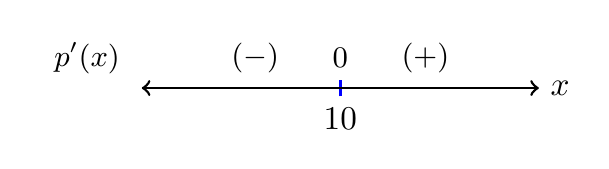
\begin{tikzpicture}[scale=1.2]
              \begin{axis}[
              axis y line=left,
            xlabel={$x$},
            ylabel={},
            xlabel style={anchor=west},
      y axis line style={draw=none},
          x axis line style={draw opacity=0},
            %grid = major,
            every major tick/.append style={ thick, blue, major tick length=5pt},
            xtick       = {0},
            xticklabels = {$10$},
            ytick       = \empty,
            yticklabels={},
                                      y  axis line style=-,
                          % y axis/.append style={y axis line style=-}
            samples     = 320,
            restrict y to domain=-40:40,
            xmin = -5.5, xmax = 3.5,
            ymin = -.5, ymax = 1,
            height=1in, width=2.75in
          ]
    \draw[thick,<->] (-3.5,0) -- (3.5,0);
     \node[anchor=west] at (-5.25,.5) {\small $p^{\prime}(x)$};
           \node at (0,.5) {\small $0$};
        \node at (-1.5,.5) {\small $(-)$};
        \node at (1.5,.5) {\small $(+)$};
          %
        \end{axis}
    \end{tikzpicture}
\end{center}
by computing $p'(9) = -2<0$ and $p'(11)=2>0$. The first derivative test lets us conclude that $x=10$ is a local minimum.

Alternatively, noting that $p''(x) = 2$ is positive at $x=10$ would also tell us that $x=10$ is a local minimum for $p(x)$.

In either case, that $p(x)$ has a single critical point which is a local minimum implies that $x=10$ minimizes $p(x)$ across the entire interval $(-\infty, \infty)$. Substituting back into our constraint we get $y=x-20 = -10$. We then conclude that the two numbers differing by 20 which have the smallest product are $10$ and $-10$, which have product $p=-100$.
}

%%%%%%%%%%%%%%%%%%%%%%%%%%%%%%%%%%%%%%%%%%%%%%%%%%%%%
%%%%%%%%%%% END PROBLEM A3 %%%%%%%%%%%%%%%%%%%%%%%%%%
%%%%%%%%%%%%%%%%%%%%%%%%%%%%%%%%%%%%%%%%%%%%%%%%%%%%%

\newpage

%%%%%%%%%%%%%%%%%%%%%%%%%%%%%%%%%%%%%%%%%%%%%%%%%%%%%
%%%%%%%%%%% BEGIN PROBLEM I2 %%%%%%%%%%%%%%%%%%%%%%%%
%%%%%%%%%%%%%%%%%%%%%%%%%%%%%%%%%%%%%%%%%%%%%%%%%%%%%
\item 

The graph of $f(x)$ is given below.

\begin{center}
    \begin{tikzpicture}[scale=1.25]
          \begin{axis}[
            xlabel={$x$},
            xtick       = {1,2,3,4,5,6,7,8},
            ytick       = {-3, -2, -1, 0,1,2,3,4},
            samples     = 320,
            domain      = -1:9.5,
            restrict y to domain=-3.5:2.5,
            xmin = -0.5, xmax = 8.5,
            ymin = -3.5, ymax = 4.5,
            height=2.1in, width=2.7in,
            grid=both, grid style=dashed
          ]
          \draw[ultra thick, blue,--] (0,2) -- (3,4) -- (6,-2) -- (8, 2);
          \node at (4,3) {$f(x)$};
          \end{axis}
    \end{tikzpicture}
\end{center}

In addition, we know that $g(x)$ satisfies the following:

\[
\int_5^3 g(x)\,dx = -2,
\qquad
\int_0^3 g(x)\,dx = 10.
\]

Find the values of the following integrals.

\begin{enumerate}

\item $\displaystyle \int_5^7 f(x)\,dx$

\vfill

\textcolor{blue}{
From the graph, $f(x)$ is linear on each interval.
On $[3,6]$, the line has equation $f(x)=10-2x$.
On $[6,8]$, the line has equation $f(x)=2x-14$.
Thus,
\[
\int_5^7 f(x)\,dx
=
\int_5^6 (10-2x)\,dx
+
\int_6^7 (2x-14)\,dx.
\]
(Break apart property)
Compute each integral:
\[
\int_5^6 (10-2x)\,dx
=
[10x-x^2]_5^6
=
(60-36)-(50-25)
=
-1,
\]
\[
\int_6^7 (2x-14)\,dx
=
[x^2-14x]_6^7
=
(49-98)-(36-84)
=
-1.
\]
Therefore,
\[
\int_5^7 f(x)\,dx = \int_5^6 f(x)\,dx + \int_6^7 f(x)\,dx = -1 + (-1) = -2.
\]
}

\vfill

\item $\displaystyle \int_3^5 \bigl(2f(x)-g(x)\bigr)\,dx$

\vfill

\textcolor{blue}{
Use linearity of the integral:
\[
\int_3^5 (2f(x)-g(x))\,dx
=
2\int_3^5 f(x)\,dx
-
\int_3^5 g(x)\,dx.
\]
From the given information,
\[
\int_5^3 g(x)\,dx = -2
\quad \Rightarrow \quad
\int_3^5 g(x)\,dx = 2. \text{ (reverse limits property) }
\]
On $[3,5]$, $f(x)=10-2x$, so
\[
\int_3^5 f(x)\,dx
=
[10x-x^2]_3^5
=
(50-25)-(30-9)
=
4.
\]
Thus,
\[
2\int_3^5 f(x)\,dx
-
\int_3^5 g(x)\,dx = 2(4)-2 = 6.
\]
Therefore,
\[
\int_3^5 \bigl(2f(x)-g(x)\bigr)\,dx = 6.
\]
}

\vfill

\item $\displaystyle \int_0^5 \bigl(2f(x)-g(x)\bigr)\,dx$

\vfill

\textcolor{blue}{
Again using linearity,
\[
\int_0^5 (2f(x)-g(x))\,dx
=
2\int_0^5 f(x)\,dx
-
\int_0^5 g(x)\,dx.
\]
Compute $\int_0^5 g(x)\,dx$:
\[
\int_0^5 g(x)\,dx
=
\int_0^3 g(x)\,dx
+
\int_3^5 g(x)\,dx
=
10+2
=
12. \text{ (break apart property) }
\]
Now compute $\int_0^5 f(x)\,dx$.
On $[0,3]$, $f(x)=2+\frac{2}{3}x$, so
\[
\int_0^3 \left(2+\frac{2}{3}x\right)\,dx
=
[2x+\tfrac{1}{3}x^2]_0^3
=
6+3
=
9.
\]
On $[3,5]$, $\int_3^5 f(x)\,dx = 4$.
Thus,
\[
\int_0^5 f(x)\,dx = 9+4 = 13.
\]
Finally,
\[
2\int_0^5 f(x)\,dx
-
\int_0^5 g(x)\,dx = 2(13)-12 = 14.
\]
Therefore,
\[
\int_0^5 \bigl(2f(x)-g(x)\bigr)\,dx = 14.
\]
}

\vfill

\end{enumerate}

%%%%%%%%%%%%%%%%%%%%%%%%%%%%%%%%%%%%%%%%%%%%%%%%%%%%%
%%%%%%%%%%% END PROBLEM I2 %%%%%%%%%%%%%%%%%%%%%%%%%%
%%%%%%%%%%%%%%%%%%%%%%%%%%%%%%%%%%%%%%%%%%%%%%%%%%%%%

\newpage

%%%%%%%%%%%%%%%%%%%%%%%%%%%%%%%%%%%%%%%%%%%%%%%%%%%%%
%%%%%%%%%%% BEGIN PROBLEM I3 %%%%%%%%%%%%%%%%%%%%%%%%
%%%%%%%%%%%%%%%%%%%%%%%%%%%%%%%%%%%%%%%%%%%%%%%%%%%%%

\item Assume $x>0$. Write down the indefinite integrals of the following expressions. 

Although no work is required, you are encouraged to include any work that shows your thought process. 

%constant, power, exponential, log, +C, algebraic manipulation

\begin{center}
        \begin{tabular}{l c l l c l}
            %
            $\displaystyle\int 9x^{10}\,dx$ & $=$ & \textcolor{blue}{\boxed{\frac{9}{11} x^{11} + C}} &
            %
            $\displaystyle\int \dfrac{1}{x^2} \,dx$ & $=$ & \textcolor{blue}{\boxed{- \frac{1}{x} + C}}\\[1in]
            %%%%%
            $\displaystyle\int \dfrac{3}{x}-2\,dx$ & $=$ & \textcolor{blue}{\boxed{3 \ln |x| - 2x + C}}&
            %
            $\displaystyle\int 2^x\,dx$ & $=$ & \textcolor{blue}{\boxed{\frac{2^x}{\ln 2} + C}}\\[1in]
            %%%%%
            $\displaystyle\int e^x+\sqrt[3]{x} \,dx$ & $=$ & \textcolor{blue}{\boxed{e^x + \frac34 x^{4/3} + C}} & 
            %
            $\displaystyle\int \dfrac{1}{\sqrt{x^5}} \,dx$ & $=$ & \textcolor{blue}{\boxed{-\frac23 x^{-3/2} + C}}\\[0.3in]
            %%%%%
        \end{tabular}
\end{center}

%%%%%%%%%%%%%%%%%%%%%%%%%%%%%%%%%%%%%%%%%%%%%%%%%%%%%
%%%%%%%%%%% END PROBLEM I3 %%%%%%%%%%%%%%%%%%%%%%%%%%
%%%%%%%%%%%%%%%%%%%%%%%%%%%%%%%%%%%%%%%%%%%%%%%%%%%%%

\newpage

%%%%%%%%%%%%%%%%%%%%%%%%%%%%%%%%%%%%%%%%%%%%%%%%%%%%%
%%%%%%%%%%% BEGIN PROBLEM I4 %%%%%%%%%%%%%%%%%%%%%%%%
%%%%%%%%%%%%%%%%%%%%%%%%%%%%%%%%%%%%%%%%%%%%%%%%%%%%%
\item For each of the following definite integrals, determine whether the Fundamental Theorem of Calculus (FTC) can be applied to evaluate. 

If so, evaluate the integral using the FTC. There's no need to simplify your final answer.

If not, clearly indicate that and explain why.

\begin{enumerate}

\item $\displaystyle \int_{-1}^{3} \left(6x^2+\sqrt[3]{x}-1\right)\,dx$

\vfill

\textcolor{blue}{
The integrand consists of a polynomial and the cube root function.
Both $6x^2$ and $-1$ are continuous for all real numbers, and $\sqrt[3]{x}$ is also continuous for all real numbers. Therefore, the integrand is continuous on the entire interval $[-1,3]$.
Hence, the Fundamental Theorem of Calculus applies.
An antiderivative of the integrand is
\[
F(x) = 2x^3 + \frac{3}{4}x^{4/3} - x.
\]
By the FTC,
\[
\int_{-1}^{3} \left(6x^2+\sqrt[3]{x}-1\right)\,dx
=
F(3)-F(-1).
\]
Thus, the value of the integral is
\[
\left(2(3)^3 + \frac{3}{4}(3)^{4/3} - 3\right)
-
\left(2(-1)^3 + \frac{3}{4}(-1)^{4/3} - (-1)\right).
\]
}

\vfill

\item $\displaystyle \int_{-1}^{3} \left(\frac{1}{x-2} - 4e^x + 2\right)\,dx$

\vfill

\textcolor{blue}{
The integrand contains the term $\frac{1}{x-2}$, which is undefined at $x=2$.
Since $2 \in [-1,3]$, the integrand is not continuous on the entire interval of integration.
Therefore, the Fundamental Theorem of Calculus cannot be applied to this integral.
}

\vfill

\end{enumerate}

%%%%%%%%%%%%%%%%%%%%%%%%%%%%%%%%%%%%%%%%%%%%%%%%%%%%%
%%%%%%%%%%% END PROBLEM I4 %%%%%%%%%%%%%%%%%%%%%%%%%%
%%%%%%%%%%%%%%%%%%%%%%%%%%%%%%%%%%%%%%%%%%%%%%%%%%%%%

\newpage

\begin{center}
{\bf DO NOT REMOVE THIS SHEET FROM YOUR EXAM PACKET}
\end{center}

\begin{center}
    \begin{tabular}{ r | c | l }
    {\bf Description} & {\bf Formula} & {\bf Variables}\\
    \hline
    area of a square & $A=s^2$ & $s=$ side length\\
    \hline
    area of a rectangle & $A=lw$ & $l=$ length, $w=$ width\\
    \hline
    area of a triangle & $A=\frac12bh$ & $b=$ base, $h=$ height\\
    \hline
    area of a circle & $A=\pi r^2$ & $r=$ radius\\
    \hline
    volume of a rectangular box & $V=lwh$ & $l=$ length, $w=$ width, $h=$ height\\
    \hline
    %volume of a circular cylinder & $V=\pi r^2 h$ & $r=$ radius, $h=$ height\\
    %\hline
    %volume of a sphere & $V=\frac43\pi r^3$ & $r=$ radius\\
    %\hline
    revenue & $R(x) = p\cdot x = p\cdot Q$ & $p=$ unit price, $x=Q=$ quantity sold\\
    \hline
    profit & $P(x) = R(x) - C(x)$ & $R(x)=$ revenue, $C(x)=$ cost\\
    \hline
    average cost & $\overline C(x) = \frac{C(x)}{x}$ & $C(x)=$ cost\\
    \end{tabular}
\end{center}

\begin{center}
{\bf DO NOT REMOVE THIS SHEET FROM YOUR EXAM PACKET}
\end{center}

\newpage

This page is left blank intentionally.\\

Use this page if you need additional space to write your solutions to any problem. \\

If you wish this page graded, you must refer to this page on \textbf{the original page} of the problem. Otherwise, your grader will NOT consider your work on this page.

\newpage

This page is left blank intentionally.\\

Use this page if you need additional space to write your solutions to any problem. \\

If you wish this page graded, you must refer to this page on \textbf{the original page} of the problem. Otherwise, your grader will NOT consider your work on this page.

\end{enumerate}

\end{document}